\squarebox[LightBlue]{
\chapterabstract{This chapter presents the methodologies and experiments used to collect datasets for training machine learning models for anomaly detection and root cause diagnosis in low-latency applications. We conduct three data collection experiments, each performed in a lab environment, with careful attention to ensuring they were both reproducible and as realistic as possible. The experiments focus on 4G networks, cloud gaming applications under emulated 4G conditions, and Cloud VR applications in Wi-Fi scenarios. These datasets form the foundation for the machine learning models developed and evaluated in subsequent chapters.}}

% The first set of experiments focused on achieving reproducible conditions for cellular networks. We collected 4G network conditions using the Saturator tool, generating transmission opportunity (txops) files that emulate realistic, time-varying network behaviors. Using these files, we collected cloud gaming datasets under emulated 4G conditions, leveraging Mahimahi-LinkShell and DECAF tools to capture detailed Quality of Experience (QoE) and Quality of Service (QoS) metrics.
% The final experiment extended the scope to Cloud VR applications operating under Wi-Fi network conditions. We conducted experiments to collect Cloud VR datasets under both normal and impaired Wi-Fi network conditions, simulating scenarios such as interference and signal attenuation.

\minitoc
%\newpage

%The techniques developed in this thesis for anomaly detection and root-cause analysis of low-latency (LL) applications require data collected from a series of controlled experiments. All experiments were conducted in a lab environment, with careful attention to ensuring they were both reproducible and as close as possible to real-world conditions.

%Given our objective of studying LL applications on networks with time-varying capacity, the first set of experiments focused on cloud gaming (CG) applications over cellular networks. To achieve reproducibility in data collection for CG on these networks, we first set up a testbed to capture 4G network conditions from Orange’s commercial network. This provided a realistic baseline of cellular network behavior. Using these recorded network conditions, the second phase of our experimentation involved collecting Key Performance Indicators (KPIs) for CG applications, allowing us to analyze Quality of Experience (QoE) degradation and performance under different network scenarios.

%The final experiment extended the scope to CloudVR gaming applications, where we studied their behavior over WiFi network.


\contributions{
The main contributions of this chapter can be summarized as follows:
\begin{itemize}
    \item We collect 4G network conditions using the Saturator tool, generating transmission opportunity (txops) files that emulate realistic, time-varying network behaviors.
    \item We collect cloud gaming datasets under emulated 4G conditions by leveraging the collected txops files, Mahimahi-LinkShell, and DECAF tools to capture detailed Quality of Experience (QoE) and Quality of Service (QoS) metrics.
    \item We extend the data collection to Cloud VR applications operating under Wi-Fi network conditions. Experiments are conducted to collect Cloud VR datasets under both normal and impaired Wi-Fi conditions, simulating scenarios such as interference and signal attenuation.

\end{itemize}
}



\section{Measurements and data collection of 4G network conditions on Orange commercial network}

\subsection{Motivation}
Controlled experiments under realistic network conditions is crucial in networking. In this thesis where performance of low-latency applications under time-varying capacity networks like cellular networks, it was important to be able to perform reproducible and realistic experiments on LL applications under cellular networks. To this end, MIT researchers developed a network emulation tool called Mahimahi % reference.
This tool offers the ability to reproduce the behavior of time-varying capacity networks using recorded transmission opportunities (\textit{txops}). However, the txops used by Mahimahi are old and not representative of current cellular network capacities. They were collected on Verizon and TMobile LTE network in 2016 with a downlink throughbout about 5-10 Mbps while the rapport of \ac{ARCEP} \cite{arcepQualitServices} of 2021 report that in France, the downlink throughput on average whatever the location or the network operator used were about 71 Mbps.  Based on this observation, it was important to collect more recent txops file to perform better evaluations.


\subsection{Measurement methodology}
\subsubsection{Mahimahi-LinkShell}
Mahimahi \cite{netravali2015mahimahi} is a framework designed to capture and replay traffic from HTTP-based applications under emulated network conditions. It operates by creating a set of Linux shells, each contained within its own network namespace, meaning that each shell has an isolated network stack with its own routes, firewall, and network devices. Mahimahi includes 04 tools such as LinkShell, RecordShell, DelayShell, and LossShell. Compared to earlier traffic capture and replay tools, Mahimahi offers several advantages: it enables multi-server emulation for web applications and provides network namespace isolation in each shell. This isolation eliminates variability caused by interference from cross-traffic, thus ensuring reproducible experiments. Additionally, Mahimahi's composability and extensibility make it a versatile tool for network research.

\begin{figure*}[!t]
    \centering
    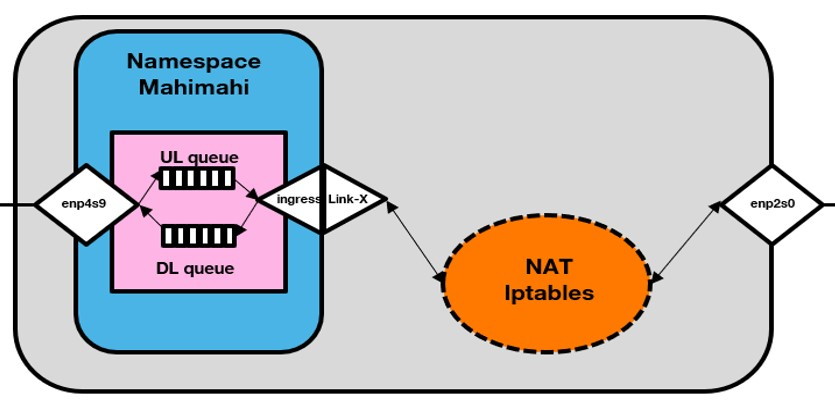
\includegraphics[width=.7\linewidth]{imgs/chapter_2/linkshell.jpg}
    \caption{LinkShell component.}
    \label{fig:chap_2:linkshell}
\end{figure*}

In this thesis, the Mahimahi component of particular interest is LinkShell. LinkShell, depicted in Fig. \ref{fig:chap_2:linkshell}, allows for the emulation of network links, either with a fixed rate or with time-varying conditions, such as those found in cellular networks. To achieve this, LinkShell relies on two transmission opportunity (txops) files: one for uplink and one for downlink network conditions. Each line in a txops file represents a transmission opportunity, defined by a time (in milliseconds) when a \ac{MTU}-sized packet (1500 bytes) can be transferred through the emulated link. Since actual packet sizes can often be smaller than 1500 bytes, a transmission opportunity may allow for the transfer of multiple packets whose combined size equals 1500 bytes. LinkShell queues incoming packets (separately for uplink and downlink) and transmits them during the corresponding transmission opportunity. If no packet is available during a transmission opportunity, that opportunity is wasted.

An example of a txops file is depicted in Fig. \ref{fig:chap_2:txop_file}

\begin{figure*}[!t]
    \centering
    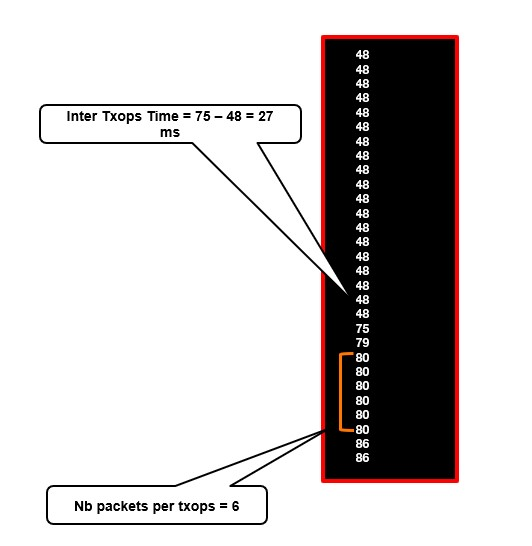
\includegraphics[width=.6\linewidth]{imgs/chapter_2/txops_file.jpg}
    \caption{An example of a txop file.}
    \label{fig:chap_2:txop_file}
\end{figure*}


% Figure with an example of a txops file

\subsubsection{Saturator Tool}
Since the existing txops files are outdated, it was necessary to collect new ones that more accurately reflect the current capacity of cellular networks. For this purpose, we utilized the Saturator tool \footnote{\url{https://github.com/keithw/multisend/blob/master/sender/saturatr.cc}}, which captures network trace samples by saturating the radio link between a User Equipment (UE) and the base station, enabling precise measurement of transmission opportunities. The operation of the Saturator tool is illustrated in Fig. \ref{fig:chap_2:saturator}. 
Our setup consisted of two Xiaomi Mi 10 5G UEs, one Ubuntu 20.04 machine acting as the client, and one Ubuntu 18.04 machine as the server. The client saturated the uplink of the USB-tethered UE, while the server saturated the downlink. Acknowledgements were exchanged between the client and server through a non-saturated WiFi-tethered UE, ensuring accurate communication without interfering with the uplink and downlink saturation. During the process, the client sent timestamped packets to the server, which computed the round-trip time (RTT) upon receiving acknowledgements. The RTT information was then used to adapt the client's congestion window, ensuring continuous saturation of the radio link. A similar process occurred on the server side to keep the radio link between the base station and UE fully saturated.

Once the capture was completed, the raw data collected by the client and server was aggregated and processed to generate two txops files (one for uplink and one for downlink). These files are used by Mahimahi’s LinkShell to emulate time-varying cellular networks, replicating the behavior observed during the experiment.

\begin{figure*}[ht]
    \centering
    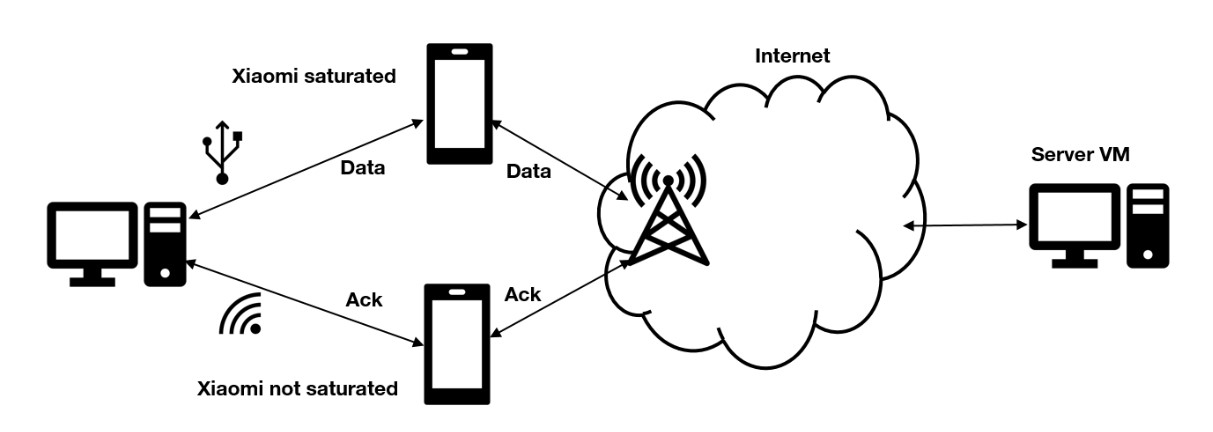
\includegraphics[width=\linewidth]{imgs/chapter_2/saturator.jpg}
    \caption{Saturator tool functioning.}
    \label{fig:chap_2:saturator}
\end{figure*}

\subsubsection{Experiments and results}


\begin{table}[!t]
\begin{threeparttable}
\caption{Characterization of the six txops captured}
\label{tab:chap_2:measurements_conditions}
\setlength\tabcolsep{0pt} % make LaTeX figure out intercolumn spacing

\begin{tabular*}{\columnwidth}{@{\extracolsep{\fill}} l c c c c c c}
\toprule
      \bf Network &  \bf  Mean & \bf Std & \bf \% of time & \bf \% of empty & \bf Location  &  \bf Hour \\
      \bf Conditions &  \bf  (Mbps)  & \bf (Mbps) & \bf $\geq 20$ (Mbps) & \bf period of 33ms & (France) &  \\
\midrule
        \bf Trace E & 230 & 48.7 & 99.9 & 2.6 & Orange Lannion & 2pm \\
\addlinespace
        \bf Trace D & 173.3 & 43.4 & 99.8 & 3.8 & Orange Lannion & 11am \\
\addlinespace
        \bf Trace C & 141.6 & 49.5 & 97.4 & 0.4 & Brélévenez & 9am \\
\addlinespace
        \bf Trace B & 78.8 & 20.3 & 99.5 & 8.0 & Brélévenez & 1pm \\
\addlinespace
        \bf Trace A & 45 & 7.4 & 99.3 & 5.8 & Plemeur-Bodou & 3pm \\
\addlinespace
        \bf Highway & 43.7 & 31.5 & 70.5 & 17.7 & Guingamp - Lannion & 10am \\


\bottomrule
\end{tabular*}
\end{threeparttable}
\end{table}
We conducted txops captures using this setup on the Orange 4G network in January 2022. Each capture lasted for 10 minutes, under varying network conditions, including differences in average bandwidth, bandwidth variability, and time gaps, to ensure the generated txops files would be representative of typical network scenarios. Additionally, we captured txops data during a mobility experiment on a highway between Guingamp and Lannion (France), traveling at 110 km/h. This capture reflected highly variable coverage, with strong signal near urban areas and weak coverage in rural zones.

As a result, six txops files (covering both uplink and downlink) were collected, representing diverse conditions of the Orange 4G network. The experimental conditions and key statistics of the recorded traces are presented in Tab. \ref{tab:chap_2:measurements_conditions}. Further details on the six txops files can be found in the appendix \ref{txops_annex}. % Add reference and figure



\takeaway{We collect in this experiment new txops files that will be used in the rest of our work for data collection on CG platforms but could also serve for other use-cases like performance evaluation of web applications under cellular network conditions \cite{mathieu2021evaluating} or for congestion control evaluation.

As such, the datasets are available as OpenData : \url{https://cloud-gaming-traces.lhs.inria.fr/ANR-19-CE25-0012_Mahimahi_Orange_4G_traces_January_2022.zip}}



\section{Data collection of user-KPI time series data for cloud gaming sessions over 4G networks}
\subsection{Motivation}
Using the six transmission opportunity (txops) files generated from the previous experiments, we conducted a series of measurements to collect datasets for cloud gaming (CG) applications operating under realistic 4G network conditions. These datasets are essential for developing machine learning (ML) models aimed at detecting \ac{QoE} degradations. By leveraging both representative network conditions and commercial CG platforms, we ensured that the collected data closely reflected real-world scenarios, making the results applicable to actual deployment environments.

\subsection{Methodology}
Our methodology for data collection relies on the integration of the Mahimahi-LinkShell tool (described earlier) and the DECAF tool, enabling comprehensive QoE and \ac{QoS} measurement for CG platforms.

\subsubsection{DECAF tool}
DECAF \cite{Iqbal2021DissectingCG} is a tool designed to measure delay and streaming performance for CG applications. While DECAF includes capabilities for game delay measurement, we focused exclusively on its streaming performance features in this work. This decision was made because the game delay measurement module is not generalizable across the range of video games used in our experiments.

The streaming measurement module of DECAF is built on an instrumentation of the WebRTC API in Chromium, extending its capabilities to collect additional metrics beyond those natively provided by the API. This enhancement allowed us to extract detailed time-series Key Performance Indicators (KPIs) relevant for QoE degradation detection,

\subsubsection{Testbed}
The testbed used for data collection is illustrated in Figure \ref{fig:chap_2:cg_testbed}. It consists of two main components:
\begin{itemize}
    \item Windows 10 laptop client: This device, equipped with the Chromium browser, is used for running and playing the games from CG platforms.
    \item Ubuntu 20.04 laptop as a network emulator: This machine runs the Mahimahi platform, serving as a controlled environment for emulating realistic 4G network conditions based on the txops files generated earlier. The network emulator connects to CG platform servers via a Fiber-To-The-Home (FTTH) Internet connection, ensuring that the bottleneck remains at the emulator rather than the \ac{WAN} interface.
\end{itemize}

During gameplay sessions, incoming uplink and downlink packets are queued within the network emulator and released by Mahimahi's LinkShell in accordance with the txops files. This configuration faithfully reproduces the time-varying behavior of 4G network conditions captured during the earlier measurements.

\begin{figure*}[!ht]
    \centering
    
\includegraphics[width=\linewidth]{imgs/chapter_2/cg_testbed.PNG}
    \caption{Cloud Gaming measurements testbed.}
    \label{fig:chap_2:cg_testbed}
\end{figure*}

We performed measurements on three major CG platforms compatible with Chromium and available in Europe during the experiment period: Google Stadia (STD), Nvidia GeForce Now (GFN), and Microsoft XCloud (XC). To maintain consistency across experiments, we selected racing games that were available on each platform:
\begin{itemize}
    \item \textit{Dirt 5} for STD
    \item \textit{TrackMania} for GFN
    \item \textit{F1 2021} for XC
\end{itemize}

Each game session lasted at least 5 minutes and was conducted under each of the six distinct 4G network conditions represented by the txops files. This ensured a diverse dataset covering various scenarios, including static and mobility-based network conditions.

During the gameplay sessions, we collected time-series features representing both QoS and QoE metrics. These included data such as bandwidth, frame rate, latency, packet loss, and other performance indicators.

\usage{
The collected datasets are used in subsequent chapters of this thesis (Chapters \ref{chap:ml_evaluation} and \ref{chap:cats}) for ML techniques for anomaly detection in multivariate time series for QoE degradation detection in CG applications.

The datasets are available as OpenData : \url{https://cloud-gaming-traces.lhs.loria.fr/ANR-19-CE25-0012_std_gfn_xc_cg_webrtc_metrics.7z}
}
% Add information on opendata plus link

\section{Data collection of CloudVR data over Wi-Fi networks}
\subsection{Motivation}
Previous experiments on CG applications conducted over cellular networks provided foundational datasets for detecting anomalies related to QoE degradation in CG sessions. However, these datasets were not suitable for performing root cause analysis, as the underlying causes of the anomalies could not be identified. This limitation stemmed from the complex and intrinsic phenomena occurring in real cellular networks, which make it challenging to isolate and attribute specific causes to each observed anomaly. Additionally, while cloud gaming is a significant low-latency application for network operators such as Orange, it primarily serves individual clients. In contrast, industry clients, who represent a major segment of the market, are more likely to leverage CloudVR for their business needs.

Given this context, we chose to focus our data collection efforts on CloudVR applications over Wi-Fi networks. This approach allows us to generate datasets that are specifically designed to facilitate root cause analysis for CloudVR performance issues. Wi-Fi networks offer the advantage of replicating real-world scenarios in controlled laboratory environments. Using Faraday cages, we can emulate various network impairments, enabling us to systematically label the collected datasets for ML training and analysis.

\subsection{Methodology}

In this section, we outline the testbed developed for CloudVR experiments, which leverages the NVIDIA CloudXR architecture to deliver immersive virtual reality experiences over wireless networks. We begin by providing an overview of the CloudVR application framework, followed by a detailed description of the testbed infrastructure and automation components.


\subsubsection{Testbed Infrastructure}

The testbed is built upon the NVIDIA CloudXR SDK, an \ac{XR} streaming platform that utilizes edge computing and cloud-based GPU acceleration to deliver high-fidelity VR experiences. The CloudXR platform streams OpenVR-based applications from a remote server to XR client devices with limited graphical capabilities, such as the untethered \ac{HMDs} Meta Quest 2 and Meta Quest 3. These devices connect to the server through various network interfaces, including Ethernet, Wi-Fi, or cellular connections.

The CloudXR architecture consists of the following key components:;
\begin{itemize}
    \item CloudXR Driver: This server-side driver streams audio and video content from XR applications (e.g., SteamVR) to the client device using network protocols like UDP. 
    \item CloudXR Client: The client-side software enables the HMD to receive and render the streamed VR content while maintaining low latency and high-quality visuals.
\end{itemize}

The CloudVR testbed infrastructure, illustrated in Fig. \ref{fig:chap_2:cloud_xr}, is designed to facilitate controlled experiments under realistic network conditions. It consists of i) a server, a high-performance machine equipped with an Intel(R) Xeon(R) W2235 CPU @ 3.8GHz with 32 GB of RAM, NVIDIA GeForce RTX 3090 Ti with 24GB,, running the CloudXR server software to render and stream VR content; ii) a thin client, the Meta Quest 2 HMD, which acts as the client device, connected wirelessly to the network and iii) a Wi-Fi \ac{AP}, a Orange commercial Livebox router that serves as the wireless bridge between the server and the HMD.

\begin{figure*}[!t]
    \centering
    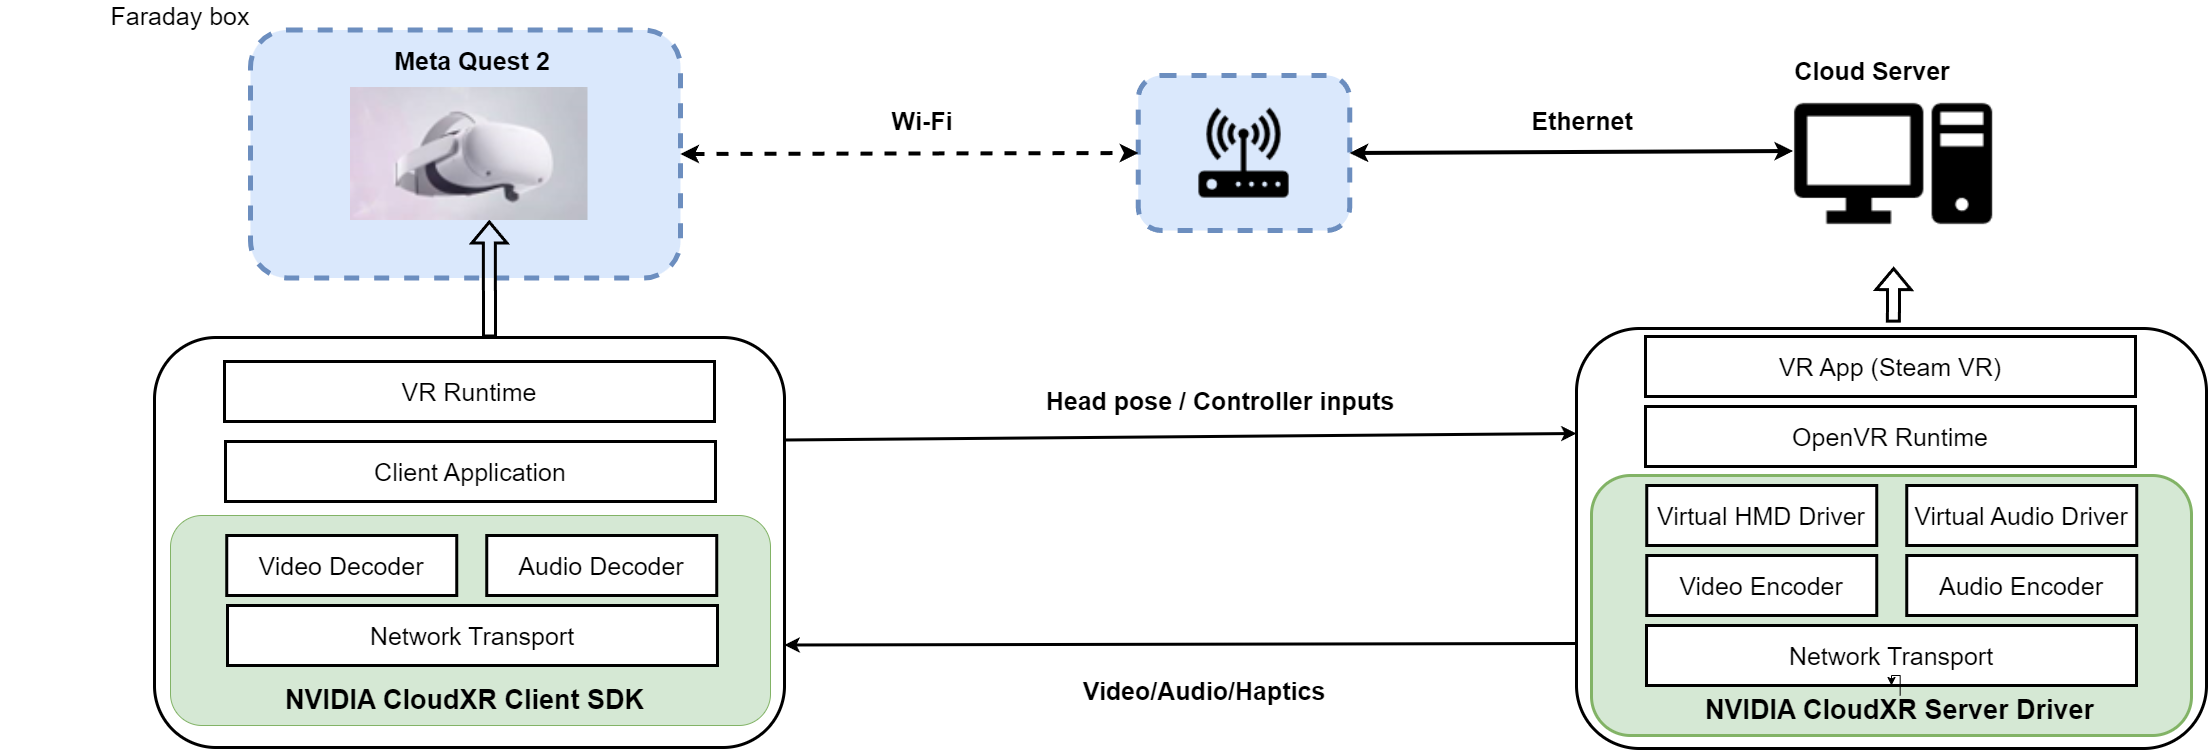
\includegraphics[width=\linewidth]{imgs/chapter_2/cloud_xr_stack.png}
    \caption{Cloud XR Architecture}
    \label{fig:chap_2:cloud_xr}
\end{figure*}


\subsubsection{Wi-Fi Testbed for Controlled Experiments}

Wi-Fi networks are critical for ensuring seamless connectivity for CloudVR applications, but they are inherently susceptible to performance degradation due to obstacles, interference, and competing traffic. To study these challenges systematically, we designed a controlled Wi-Fi testbed, as illustrated in Fig. \ref{fig:chap_2:wifi_testbed}. This setup allows for the reproduction of real-world scenarios and controlled network impairments in laboratory conditions, enabling detailed analysis of their impact on CloudVR services.

The testbed consists of two primary layers:
\begin{itemize}
    \item \textbf{Infrastructure layer:} This layer includes up to four Faraday cages used to isolate equipment from external electromagnetic interference. The cages are allocated as follows: one for the VR headset, two for the APs, and one for a station used in interference scenarios. The layer also includes two access points (AP1 and AP2): AP1 is utilized for normal and coverage experiments, while AP2 introduces interference in specific scenarios. The Faraday cages are interconnected using coaxial cables to transmit Wi-Fi signals, and \ac{RF} attenuators \footnote{\url{https://adauratech.com/attenuators/}} are employed to simulate variations in signal strength during experiments. Two servers are part of this setup: the first server (see Fig. \ref{fig:chap_2:cloud_xr}) runs the CloudVR software and is connected to AP1 via Ethernet, while the second server acts as a traffic generator connected to AP2, simulating competing downlink traffic using UDP.

    \item \textbf{Control and Automation layer:} This layer includes a VR PC controller connected to the VR headset via USB, responsible for managing headset settings and collecting performance metrics, such as KPIs from OVR Metrics tools\footnote{\url{https://developers.meta.com/horizon/downloads/package/ovr-metrics-tool/}} or quality-of-service (QoS) statistics from CloudXR. The controller also automates game sessions using the Meta Quest Autodriver\footnote{\url{https://developers.meta.com/horizon/documentation/unity/ts-autodriver}}. Additionally, this layer features an attenuator controller that configures and manages RF attenuators via APIs, enabling automated signal attenuation adjustments through FastAPI \footnote{\url{https://fastapi.tiangolo.com/}}. Furthermore, the Livebox controller manages the Livebox via Telnet to collect Wi-Fi KPIs every 3 seconds. A local ELK Stack \footnote{\url{https://www.elastic.co/fr/elastic-stack}} database aggregates data from all controllers for post-experiment analysis.

\end{itemize}

\begin{figure*}[!t]
    \centering
    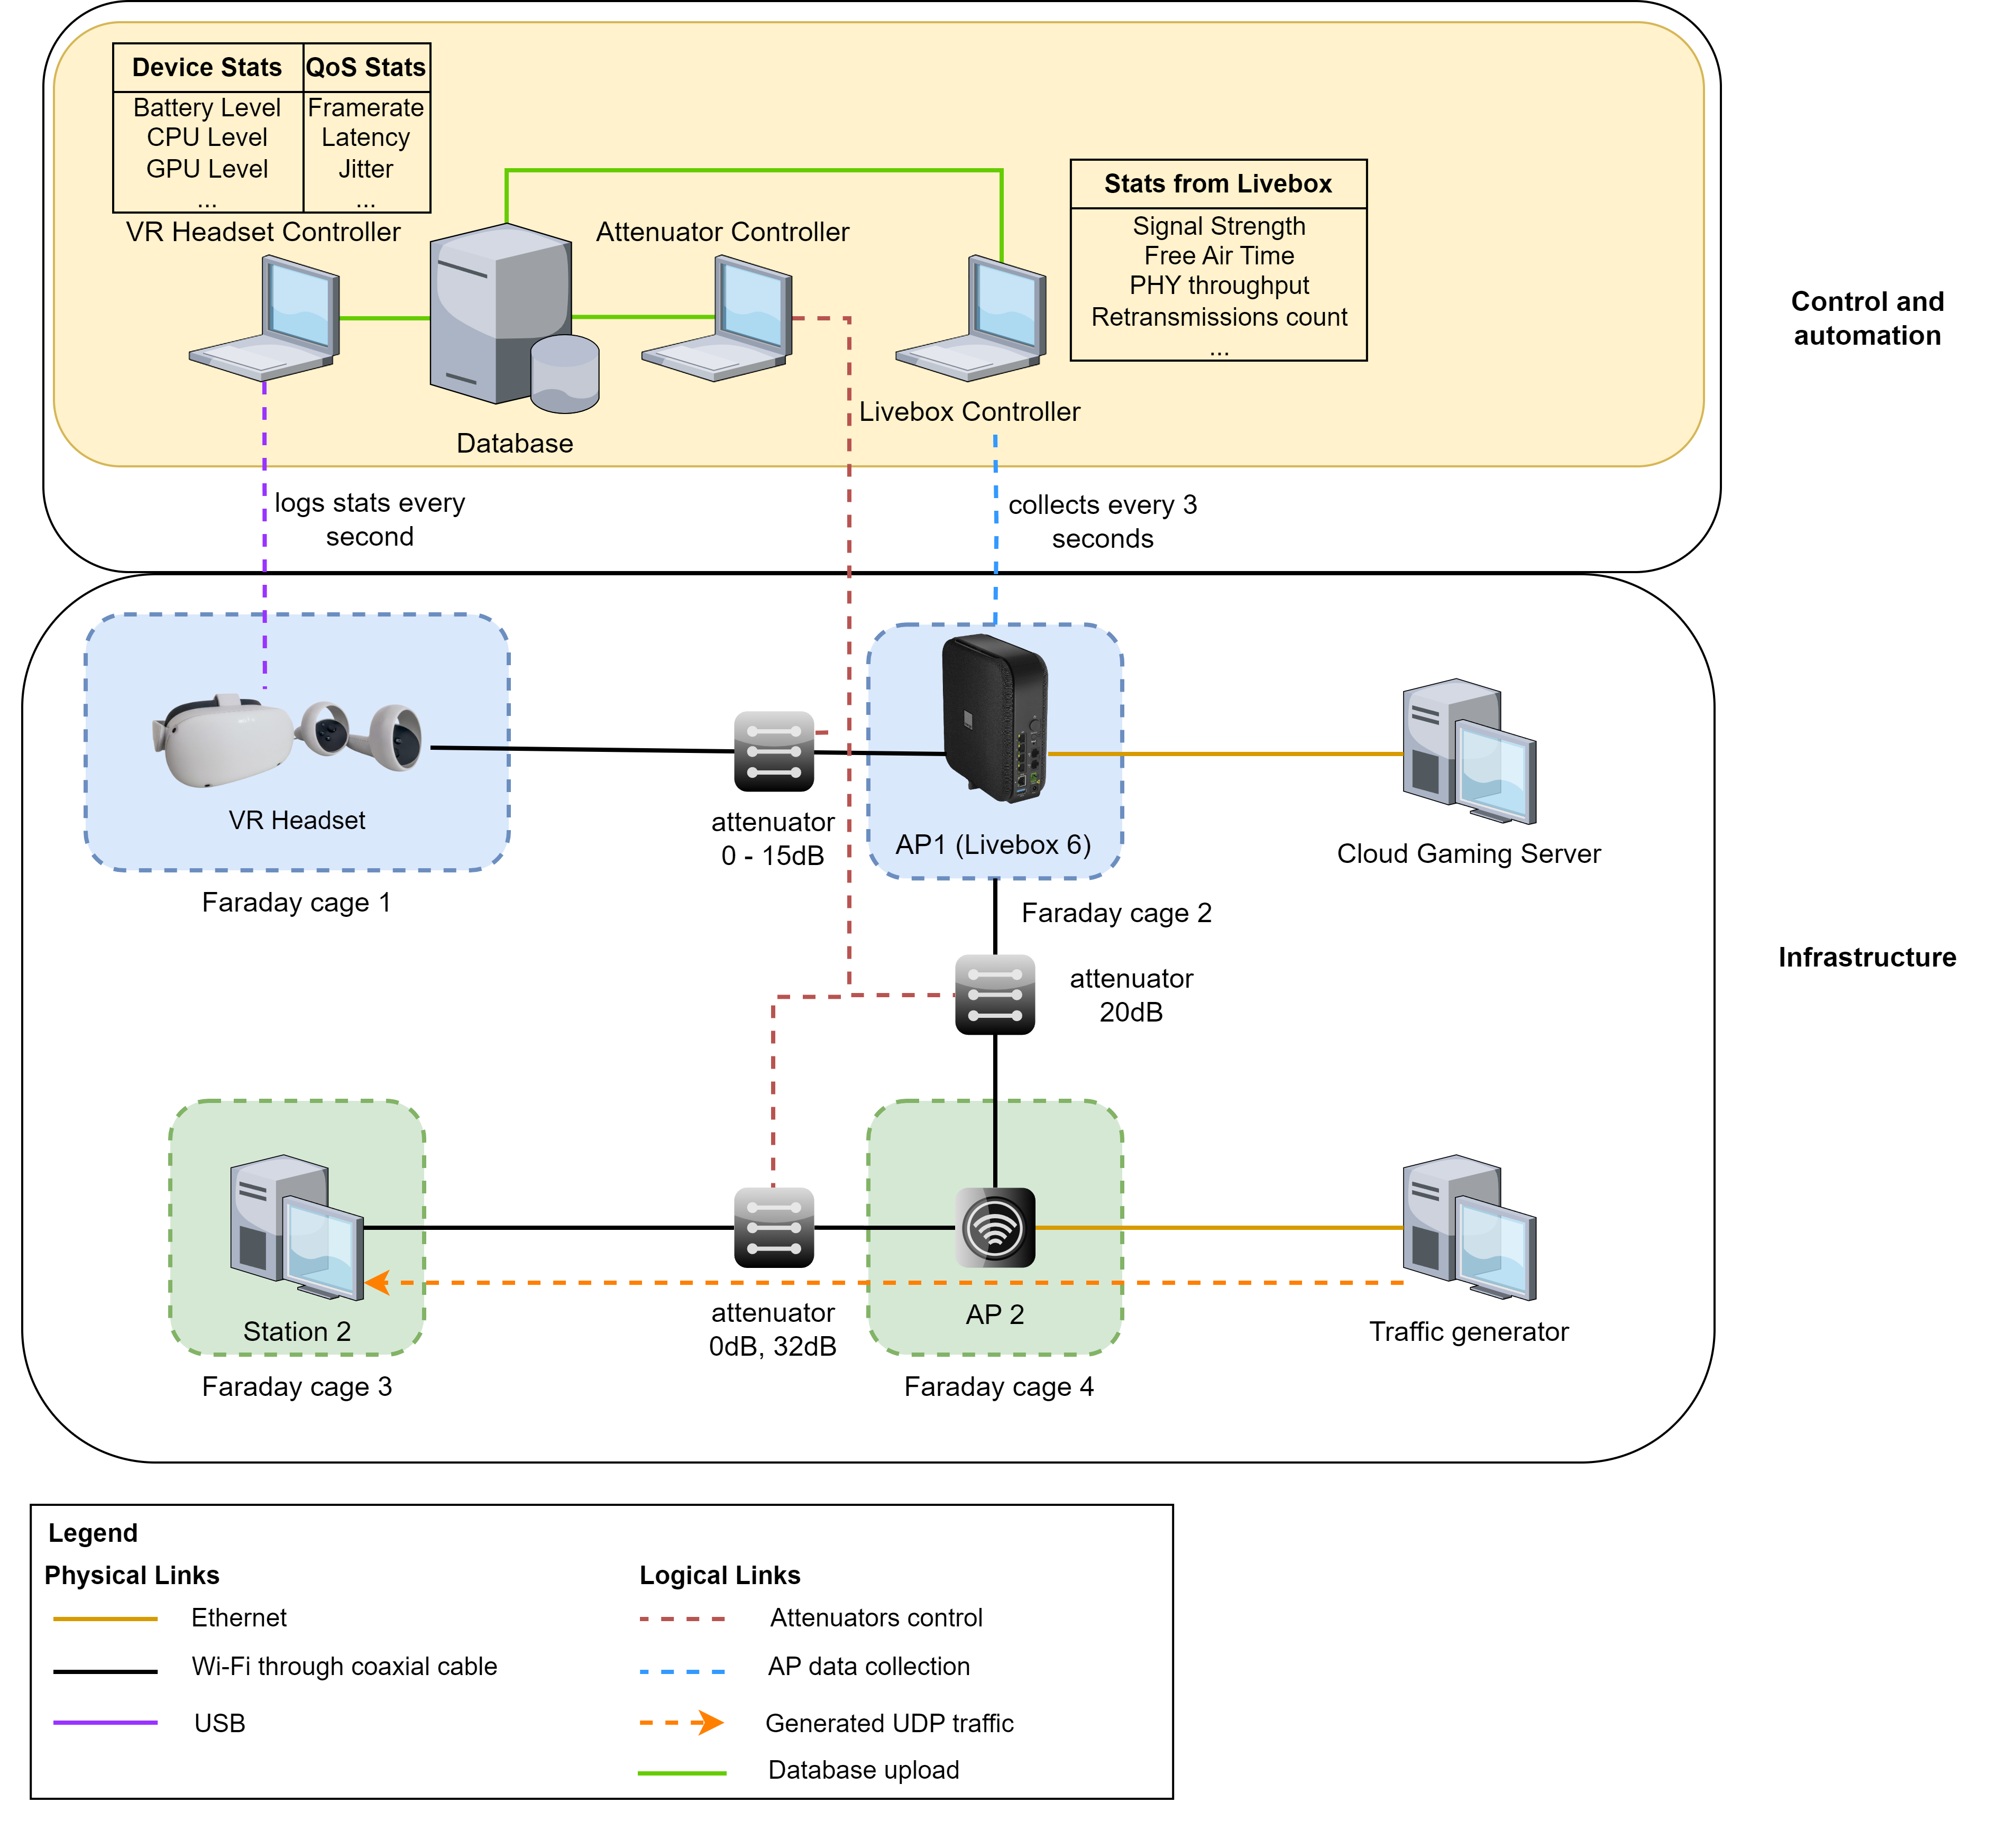
\includegraphics[width=\linewidth]{imgs/chapter_2/WiFi_testbed.png}
    \caption{Wi-Fi testbed architecture}
    \label{fig:chap_2:wifi_testbed}
\end{figure*}

\subsubsection{Scenarios considered}

We collect Cloud VR data across several controlled scenarios using the Beat Saber game as a benchmark. These scenarios were executed on both the 2.4 GHz and 5 GHz frequency bands, as detailed below:
\begin{itemize}
    \item \textbf{Normal scenarios :} CloudVR sessions were conducted under ideal conditions, without any Wi-Fi impairments. The VR headset was positioned in an optimal coverage area and connected to the primary access point (AP1) for each frequency band. A total of 5 sessions, each lasting 300 seconds, were performed for both the 2.4 GHz and 5 GHz bands.
    \item \textbf{Coverage scenarios :} To evaluate the impact of signal strength variations, an RF attenuator was used to simulate different received signal strength indicator (RSSI) values during VR sessions agter launching the game. RSSI levels of \{-55 dB, -60 dB, and -65 dB\} in 2.4 GHz and RSSI levels of \{-80 dB, -85 dB, and -90 dB\} in 5GHz. Each configuration was tested in three sessions, with each session lasting 100 seconds.

    \item \textbf{Interference scenarios :} Interference was introduced by a neighboring station connected to a secondary access point (AP2) operating on the same frequency and bandwidth as AP1. The interference was simulated by occupying a portion of the transmission opportunities (txops) available on AP1 after starting the game. Interference levels leaving \{10\% and 15\%\} of txops in 2.4 GHz band and interference levels leaving \{9\%, 10\%, and 11\%\} of txops in 5GHz for AP1. Each configuration was tested in three sessions, with each session lasting 100 seconds.
\end{itemize}

The testbed configuration ensures a highly controlled environment for Cloud VR experiments. By utilizing Faraday cages, we eliminate uncontrolled radio interference, and by deploying local servers, we remove fluctuations from external network segments. Automation allows for the seamless execution of test scenarios and comprehensive data collection of Cloud VR applications.




\subsubsection{Data collected}

During the Cloud VR experiments, three distinct types of data were collected to comprehensively capture application performance and network behavior:
\begin{itemize}
    \item \textbf{Application-Level Metrics}: Metrics were obtained directly from the Oculus OVR Metrics Tool, which provides detailed insights into the performance of the VR application on the headset. These include frame rates, resolution, CPU and GPU levels and usage, and other statistics related to VR streaming. These metrics help evaluate the QoE from the perspective of the end user. Additionally, QoS metrics were retrieved from the NVIDIA CloudXR stack, which facilitates the streaming of high-quality VR content from the server to the headset. These metrics include network round trip delay, client queuing time, packet loss, and jitter.
   \item \textbf{Livebox-Level Metrics}: The collected Wi-Fi KPIs include metrics from the Wi-Fi physical layer, such as \ac{RSSI}, background noise levels, free airtime, \ac{MCS} index, channel bandwidth, and physical layer bitrates, as well as metrics from the network layer, such as data bitrates, dropped and retried packets, and packet counters for the \ac{BSS}. These metrics were collected directly from the proprietary Livebox router to monitor and evaluate the Wi-Fi conditions experienced during the Cloud VR sessions.
   \item \textbf{Raw Traffic Captures}: \ac{PCAP} data was collected using a probe placed in the Faraday cage near the VR headset. These raw traffic captures provide a detailed view of packet-level interactions between the VR client and the server, including timestamps, protocol usage, packet sizes, and packet inter-arrival times, which may be useful for detecting potential anomalies at the transport and application layers.
\end{itemize}


\usage{For the experiments presented in this work, the \ac{RCD} focused solely on the Livebox-level metrics. These metrics were used to detect and classify anomalies affecting the Wi-Fi performance during Cloud VR sessions. The application-level and raw traffic metrics, while not utilized in the current analysis, present opportunities for future work. They could enhance diagnostic performance by providing richer context and additional data points for identifying the underlying causes of performance degradation.

The datasets will be available as OpenData.}



